\documentclass[10pt, onecolumn, draftclsnofoot, letterpaper,compsoc]{IEEEtran}
\usepackage[utf8]{inputenc}
\usepackage{import}
\usepackage{natbib}
\usepackage{graphicx}
\usepackage{amsmath}
\usepackage{algorithm}
\usepackage{float}
\usepackage[noend]{algpseudocode}

\bibliographystyle{plain}

\title{Capstone Design Document}
\author{GFR Group \\
        CS461 Senior Software Engineering Project \\
        Fall 2018 \\
        \today}

% creates keywords for input and output in algorithm block
\algblock{Input}{EndInput}
\algnotext{EndInput}
\algblock{Output}{EndOutput}
\algnotext{EndOutput}
\newcommand{\Desc}[2]{\State \makebox[13em][l]{#1}#2}

\begin{document}

\maketitle

Autonomous vehicles require robust internal representations of the world in order to make correct driving decisions. Information from multiple sensor modalities including camera, lidar, and odometry must be utilized in order to create a map of the world and localize the vehicle within that map. This document covers the design methodology used to develop a driverless formula-style racing car. The racing car will be entered into driverless racing competitions starting in 2019.

\newpage
\tableofcontents
\newpage

\section{Introduction}

\subsection{Terminology}

\begin{itemize}
    \item \textbf{Lidar} A visual sensor that fundamentally works like a radar but uses lasers instead of radio waves
    \item \textbf{GPS} Global Positioning System. Device used to a estimate longitudinal and latitudinal coordinates of the vehicle.
    \item \textbf{DGPS} Differential GPS. Device used to estimate relative change of position over time.
    \item \textbf{IMU} Inertial Measurement Unit. Device used to estimate the velocity of the vehicle.
    \item \textbf{ROS} Robot Operating System. Software used to manager subsystems of an autonomous agent.
    \item \textbf{Faster RCNN} Faster Region-based Convolutional Neural Network. Machine learning model used to localize objects in an image.
    \item \textbf{YOLO} You Only Look Once. Machine learning model used to localize objects in an image.
    \item \textbf{SSD} Single Shot Multibox Detector. Machine learning model used to localize objects in an image.
    \item \textbf{SLAM} Simultaneously Localization And Mapping. Algorithm for mapping the surroundings of an agent and localizing that agent within the map.
    \item \textbf{GFR} Global Formula Racing. International formula racing cooperation between OSU and DHBW.
    \item \textbf{DHBW} Duale Hochschule Baden-Wurttemberg. University located in Stuttgart, Germany
    \item \textbf{OSU} Oregon State University. University located in Corvallis, Oregon
    \item \textbf{EKF} Extended Kalman Filter. Algorithm for approximating the behavior of a function.
    \item \textbf{RANSAC} Random Sample Consensus. Algorithm for approximating the behavior of a function.
\end{itemize}

% REQUIREMENTS OF DOCUMENT
% describe plan for project
% include any technologies, methods, parts and designs


\subsection{Purpose}
% high level overview of the competition and vehicle
 The driverless vehicle must utilize sensor input from camera, lidar, GPS, and IMU in order to construct a virtual representation of the world around it as well as localize itself within that world. The virtual representation of the world is then used to compute the optimal path and trajectories needed maneuver around a track. The driverless vehicle is expected to compete in the Formula SAE (FSAE) competition in August 2019. 

\subsection{Scope}
% high level overview of the vision system
Our team is tasked with constructing the vision, odometry, mapping, and localization systems for a driverless formula style racing car for the Global Formula Racing (GFR) team. The purpose of our system is to create a robust virtual representation of the vehicle's environment. Algorithms will be developed for detecting the location and color of the cones using lidar and camera. The cone locations and colors will be used to construct a dynamic map of the world, updating the map as the vehicle moves and new cones are seen. As the vehicle moves, our system will need to use positional data from the GPS and IMUs in order to update the position of the vehicle within the map. 

\subsection{Stakeholders}
The stakeholder of this system is the Global Formula Racing team. GFR will use the system described in this document to participate in international driverless racing competitions.

\newpage
\section{Design Components}

% ===================================
%               CAMERA 
% ===================================

\subsection{Camera}
\subsubsection{Design View} % Basically high-level introduction

% Primary goals of camera
%%% Accurately localize and classify cones in image and determine their location relative to the vehicle.
%%% Track correspondence between cones in separate frames
The camera vision system should be able to accurately detect all cones within a sufficient distance from the camera. 

\begin{figure}[H]
\centering
\label{fig:CameraExample}
\caption{Camera Cone Detection in action}
\includegraphics[width=15cm]{images/camera_cones_detected}
\end{figure}

\subsubsection{Design Viewpoints} % How our system functions and interact with users as a whole
% Describe the Functions of the system (logical flow of the algorithm.)
% Describe the Structure of the system
The vision system will be contained within a ROS node which takes in individual frames and outputs the color of each cone, the mean x and y locations of all cones, as well as the standard deviation of the cone's location in the x and y direction. The x and y locations returned will represent the position of each cone relative to the vehicle. Covariance of x and y coordinates will also be computed. Once cones have been detected, they will be published to the camera\_stream topic for use by other parts of the system. 

\begin{figure}[htbp]
\centering
\label{fig:CameraInterfaceOverview}
\caption{Camera Functional Overview}
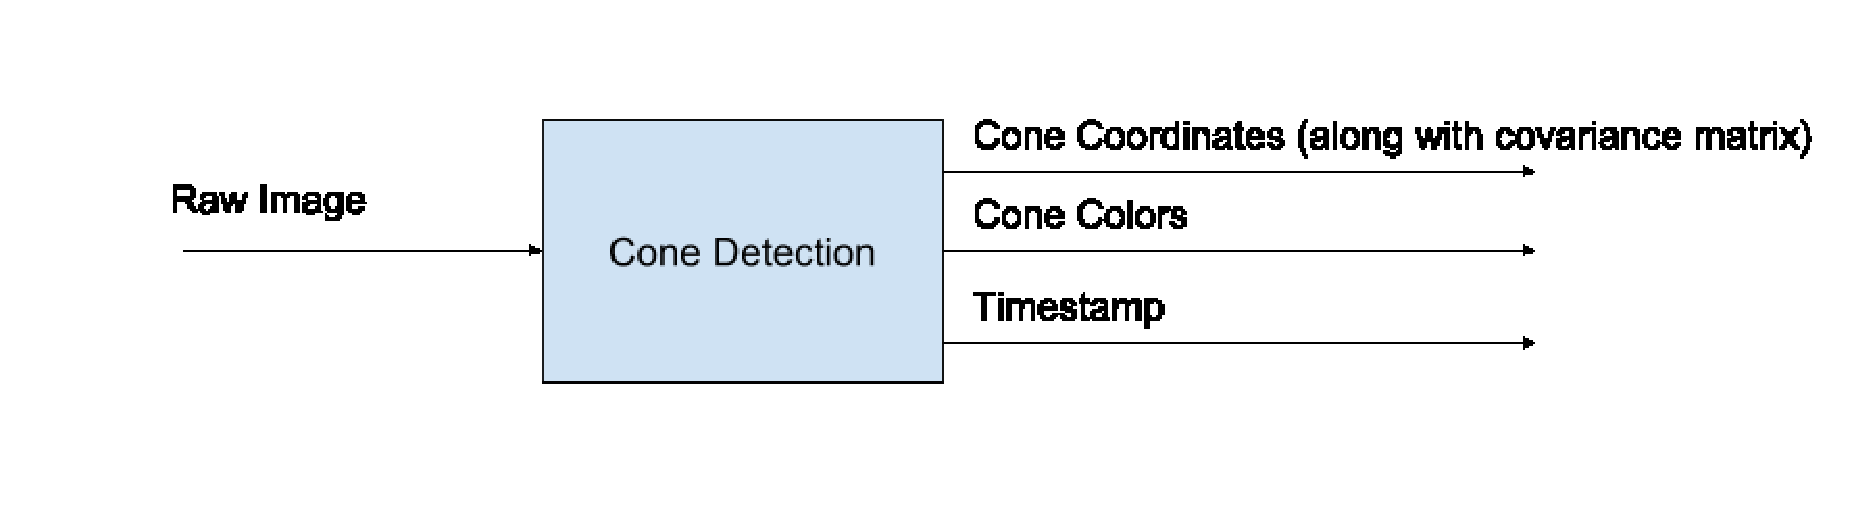
\includegraphics[width=15cm]{images/camera_cone_detection_interface}
\end{figure}

\subsubsection{Design Elements} % How we accomplish the Design Viewpoints above (This is the main part)

The cone detection model will consist of a pair of Convolutional Neural Networks, a large, accurate network, and a small, fast network. The networks will operate in tandem. The larger network will operate at a slower prediction rate, generating more accurate predictions at longer distances, while the smaller network operate at a faster prediction rate, generating less accurate predictions at longer distances but which does well detecting cones that are closer to the vehicle. Details of the algorithm are shown in algorithm \ref{alg:cameraConeDetector}.

The neural networks used for cone detection will be Faster RCNN with a ResNet-style backbone and Feature Pyramid Network. ResNet-style backbone will consist of several stages of the original ResNet. The smaller network will have less convolutional filters per layer as well as using less stages instead of than what is typically recommended.

In order to utilize a Faster RCNN model, the model must be trained on a dataset of blue, yellow, and orange traffic cones. The dataset should contain a minimum of 100 ground truth images containing at least 250 blue and yellow cones and 60 orange cones.

%%% Takes in raw image from camera_stream
%%% Preprocess image to necessary input conditions for neural network
%%%%% convert image to HSV and remove the value (v) channel
%%%%% normalize image based on the color intensity of a white region of the vehicle's hood. 
%%%%% remove region of image that likely will not ever contain cones. (the upper third of the image and in the center bottom region where the vehicle will be visible) reducing the region sized used to detect objects will result in less total computation.
%%% Send image through neural network and get bounding box and color prediction
%%% Translate bounding box predictions from pixel space to euclidean coordinates relative to vehicle
%%%%% template matching will be used to determine distance of each cone. because the cones have a fixed size, a cone that is X inches tall will be Y meters away.
%%% track features within current set of bounding boxes until inference on new image has occurred
%%% Output cone locations, cone colors, and time-stamp of when image was taken


\subsubsection{Design Rationale} % Rationale behind our Design Element above (Why we chose the above implementation)
The dual network structure for cone detection allows the vehicle to balance short-term and long-term planning of the vehicle's route. While the large network can determine twists and turns in the track from farther away, the small gives the system quick updates about what is directly in front of the vehicle. The choice to use Faster RCNN was made due to the accuracy of Faster RCNN compared to other object detection models. While models such as YOLO and SSD perform faster, the bounding box predictions of these models are less accurate. These models also perform poorly on objects at longer distances, which is crucial to accurately planning the vehicle's route from farther away.

\subsubsection{Design Tools} % What languages/packages/frameworks are used to accomplish our Design Element above
The latest versions of Pytorch and Caffe2 will be used as our machine learning framework. Facebook Research Group's Detectron, an open source implementation of Faster RCNN, will be used as our object detection model. ROS nodes will be used for data transfer between the cone detection node and other parts of the driverless system. 

\begin{algorithm}[H]
\caption{Cone Detector}
\label{alg:cameraConeDetector}
\begin{algorithmic}[1]
\import{algos/}{algo_cone_detector.tex}
\end{algorithmic}
\end{algorithm}


% ===================================
%               LIDAR 
% ===================================
\newpage

\subsection{Lidar}
\subsubsection{Design View} % Basically high-level introduction
Mounted on the chassis of the car, the lidar scans the surrounding physical environment of the car. From the scanned data, the ROS node detects and calculates the location of cones relative to the car as well as estimates the color of cones based on intensity values of the laser scans corresponding to those cones.

\begin{figure}[htbp]
\centering
\label{fig:LidarInterfaceOverview}
\caption{Lidar Cone Detection in action}
\includegraphics[width=15cm]{images/LidarSimulated}
\end{figure}

\subsubsection{Design Viewpoints} % How our system functions and interact with users as a whole
% Describe the Functions of the system (logical flow of the algorithm.)
In overview, our lidar ROS node receives 3D point cloud data from the lidar laser sensor and gives 3 outputs: first, the 2D location of the cones relative to the car; second, a covariance matrix describing how certain our 2D location is; and third, a timestamp on when the lidar point cloud was originally captured. 

\begin{figure}[htbp]
\centering
\label{fig:LidarInterfaceOverview}
\caption{Lidar Functional Overview}
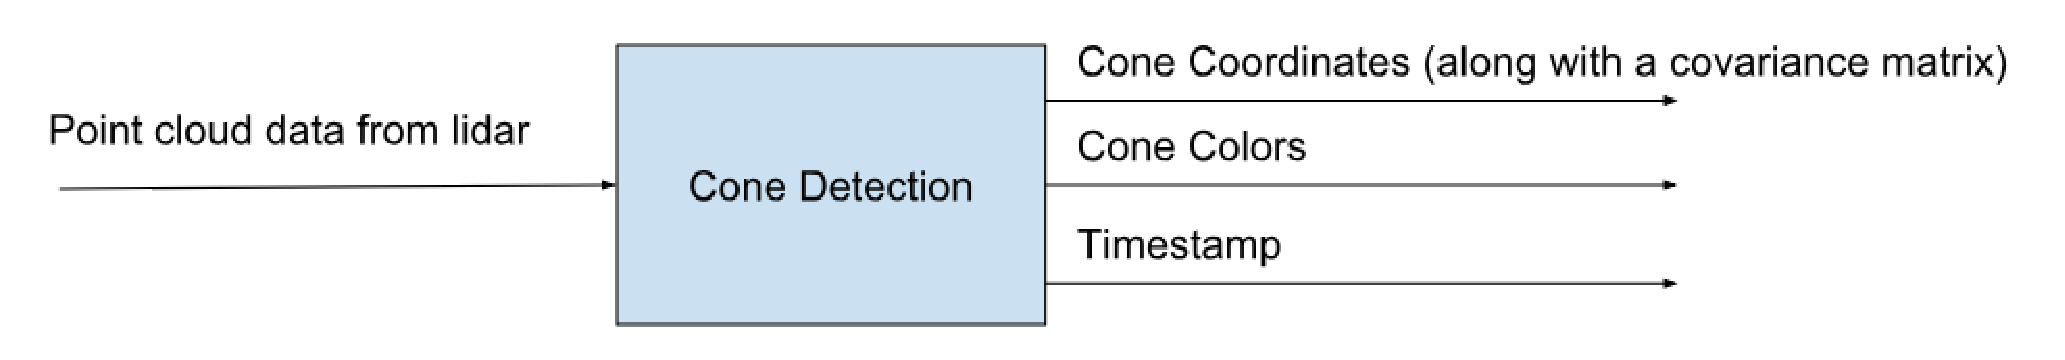
\includegraphics[width=15cm]{images/LidarInterfaceOverview}
\end{figure}

The lidar sensor continuously scans the physical environment around the car as the car is moving at a speed of at most 60 miles per hour until being turned off. Point cloud data from the lidar sensor is then published to lidar processing node in ROS. In real time, the lidar processing node differentiates between points that are cones and points that are not cones. The lidar processing node then computes the 2D coordinate of the cones relative to the physical location of the lidar sensor mounted on the car. And finally, the lidar processing node predicts and differentiates between the different colors of detected cones based on their position relative to the lidar sensor and the intensity values of the points in the point cloud corresponding to those cones.

\begin{figure}[htbp]
\centering
\label{fig:LidarInterfaceOverview}
\caption{Lidar Detailed Interface Design}
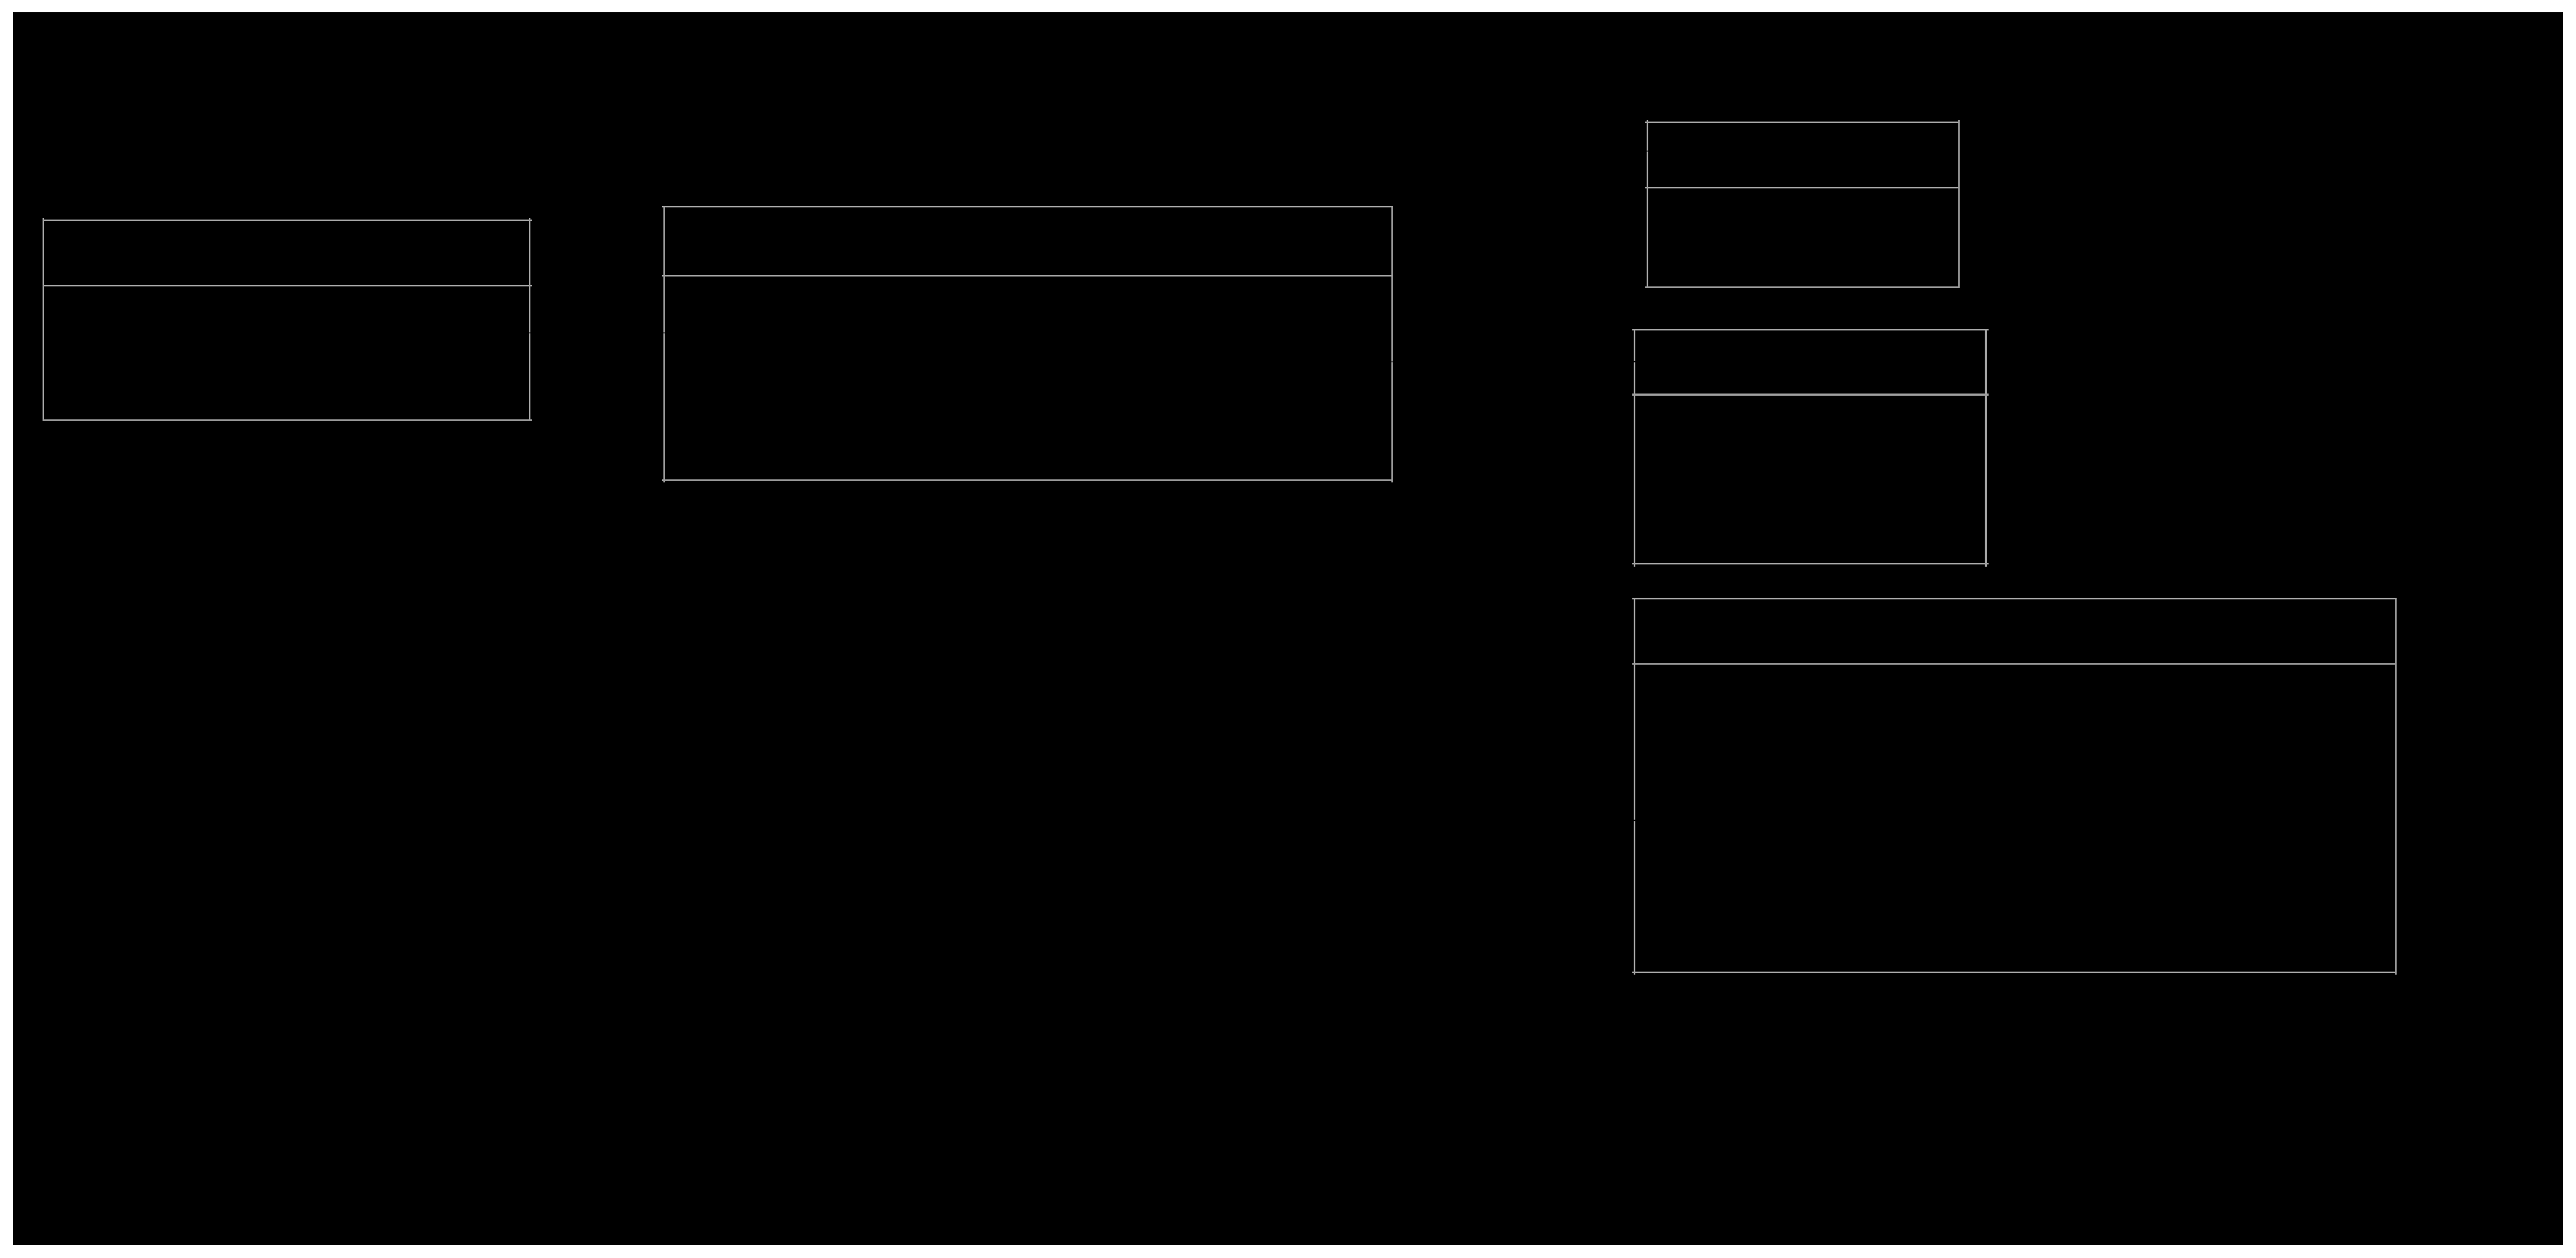
\includegraphics[width=18cm]{images/LidarInterfaceDetails}
\end{figure}

\subsubsection{Design Elements} % How we accomplish the Design Viewpoints above (This is the main part)
We use 3D hough transform to find the ground plane. After removing the ground plane, RANSAC is used to fit a cone model to cones located in the point cloud.

\begin{figure}[htbp]
\centering
\label{fig:LidarPipeline}
\caption{Lidar Processing Pipeline Diagram}
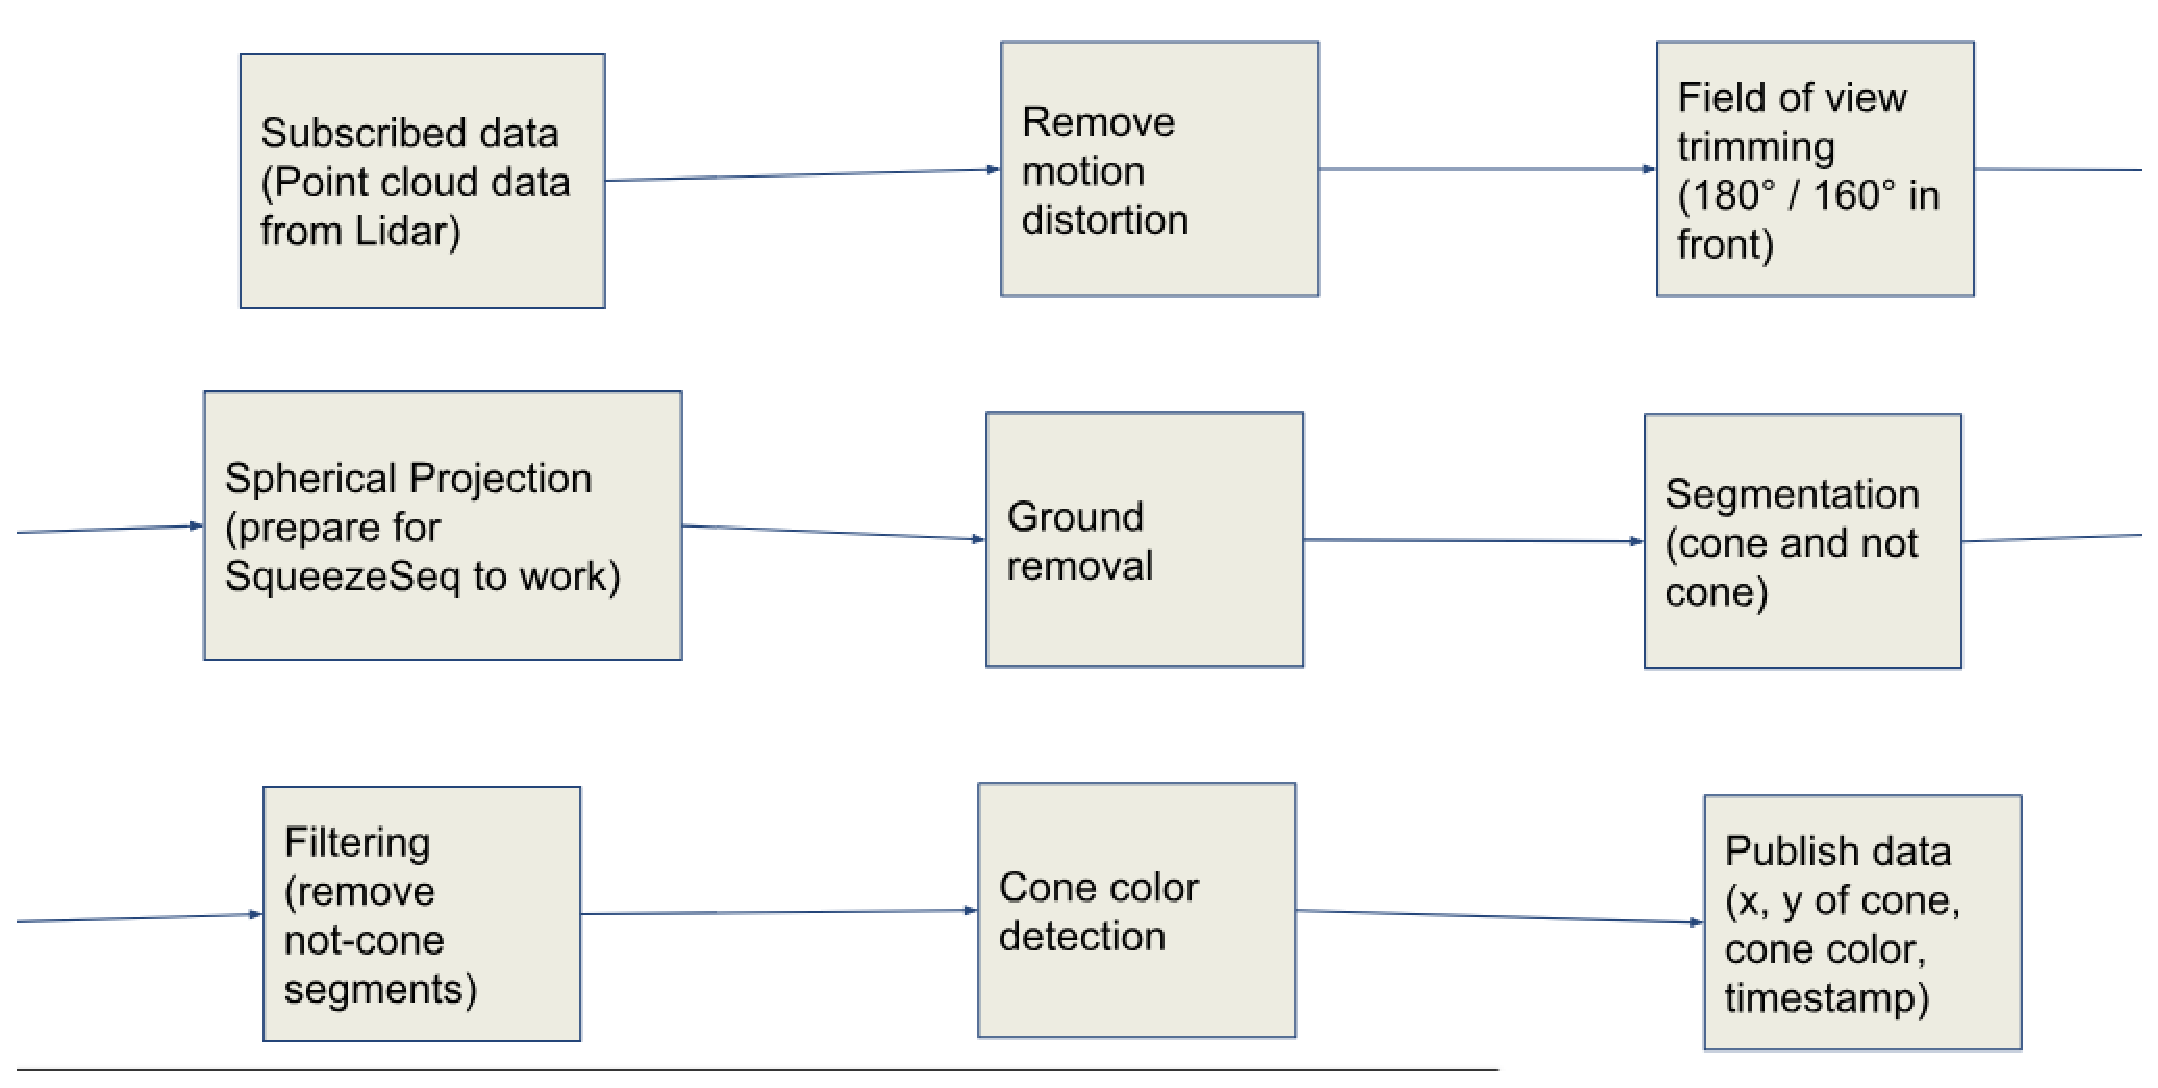
\includegraphics[width=15cm]{images/LidarPipeline}
\end{figure}


\subsubsection{Design Tools} % What languages/packages/frameworks are used to accomplish our Design Element above
We use ROS for our robotics platform and use C++ to implement our algorithms except our machine learning algorithms which we implement in Python. We use rviz to visualize our lidar scanning output overlayed with the cone detection output which are boxes surrounding the 3D model of cones.

\subsubsection{Design Rationale} % Rationale behind our Design Element above (Why we chose the above implementation)
We remove the ground plane because it does not give us any valuable information about our surrounding and also to the computational cost needed to detect cones. Because the shape of the cones is static, using a cone model to fit cones in the point cloud using RANSAC will be highly efficient.

We decided not to use the state-of-the-art, neural-network-based  algorithm, SqueezeSeg, for real-time 3D point cloud object clustering because SqueezeSeg is designed and implemented for general object detection on the real life street traffic problem. Our problem is much less complicated. Thus, SqueezeSeg is probably too complicated for what we need in our problem, which is just fixed-size, stationary, small number of cones ahead of the car.

For our programming language decision, there are two major options: Python and C++. Because the scanning data from the lidar (hardware) must be processed by a lidar processing algorithm in real time, a major concern of our system is efficiency. ROS can work with both Python and C++, however most existing implementations of relevant algorithms in the ROS ecosystem are written in C++. Python will help us get the prototype up and running quickly, and also most of machine learning model implementations and deployment pipelines are written in Python.  Therefore, we believe that the best course of action will be to do initial development in Python and rewriting all performance critical elements in C++ after our solution and been evaluated.

\newpage
% ===================================
%               ODOMETRY 
% ===================================

\subsection{Odometry}
\subsubsection{Design View} % Basically high-level introduction
The odometry system will use information from three IMUs and one GPS present on the car to determine where the car is and how fast it is moving.

\subsubsection{Design Viewpoints} % How our system functions and interact with users as a whole
% Describe the Functions of the system (logical flow of the algorithm.)
% Describe the Structure of the system
The filtered sensor data from the car will be used to determine how the car has moved over the course of the previous time step. The motion of the car will then be put through a particle filter to account for kinematics, commands, and uncertainty in sensor measurements. The change in location data will be sent to SLAM, and velocity will be sent to the dynamic controllers system. 

\subsubsection{Design Elements} % How we accomplish the Design Viewpoints above (This is the main part)
Each movement through a time step will be modeled by a rotation from the start, a translation along the new heading, and a second rotation, as shown in figure \ref{fig:motionModel}. These three parameters are all that is needed to describe an arbitrary translation and rotation through space. A particle filter will be used to fuse the IMU and GPS sensor data into a single model, where it will be sent to the SLAM system for use in their localization algorithm. A high level algorithm of a particle filter is shown in algorithm \ref{alg:particleFilter}.

\begin{figure}[htbp]
\centering
\label{fig:motionModel}
\caption{Model of a movement across a time step}
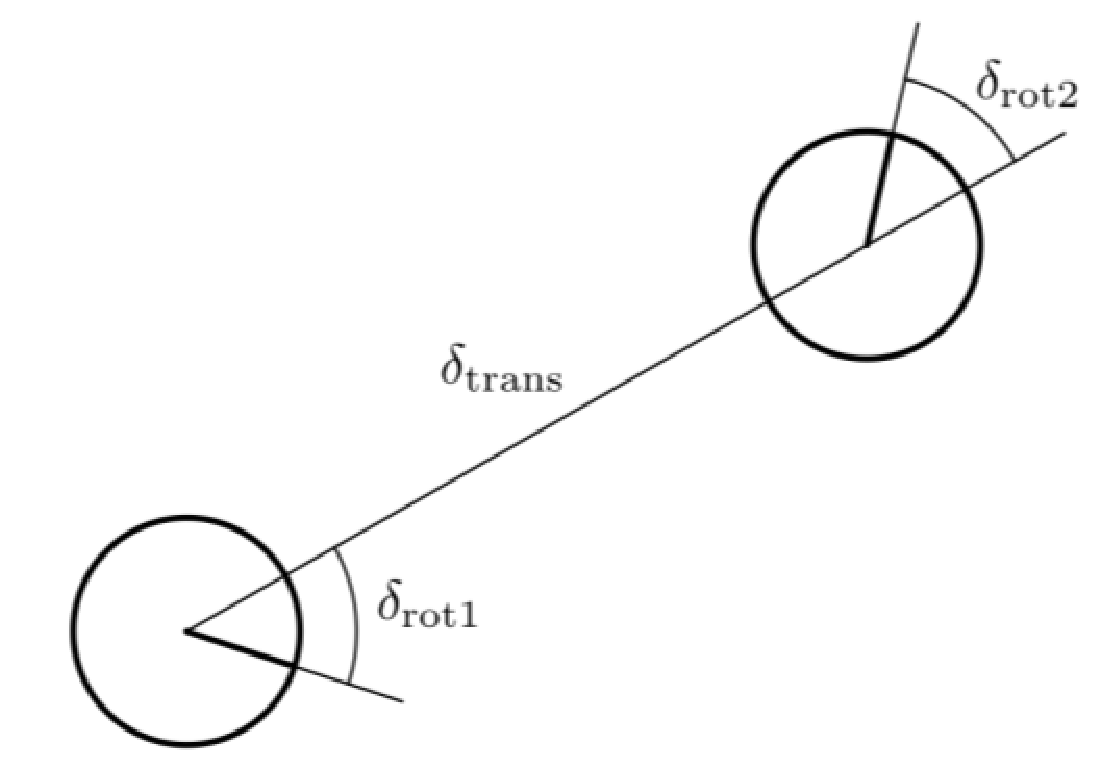
\includegraphics[width=7cm]{images/motionModel}
\end{figure}

\subsubsection{Design Rationale} % Rationale behind our Design Element above (Why we chose the above implementation)
Because SLAM will be implementing localization, it is redundant to determine absolute position in odometry as well. Therefore the minimum amount of information needed by the SLAM is how one location changes to become the next measured location, resulting in the decided upon model. The particle filter implementation was chosen because of the nonlinear nature of the sensors and model at work, and because it tends to be the most robust statistical filter implementation available. 

\subsubsection{Design Tools} % What languages/packages/frameworks are used to accomplish our Design Element above
ROS includes an odometry message which contains most of what is needed in our description of how the robot has moved. The final iteration of the message type passed to SLAM will include additional fields. The implementation will be done in Python, because this is one of the less computationally intensive components of the driverless system. NumPy will be needed for developing the system propagation and control model.

\begin{algorithm}
\caption{Particle Filter}
\label{alg:particleFilter}
\begin{algorithmic}[1]
\import{algos/}{algo_particle_filter.tex}
\end{algorithmic}
\end{algorithm}

\newpage

% ===================================
%               SLAM 
% ===================================

\subsection{SLAM}
\subsubsection{Design View}
The overall SLAM system will be able to map the surroundings of the car using cones as landmarks. It will also localize the car within the map. 
\subsubsection{Design Viewpoints} % How our system functions and interact with users as a whole
% Describe the Functions of the system (logical flow of the algorithm.)
% Describe the Structure of the system
The first step is open loop SLAM, followed by loop closure detection, and finally closed loop localization. Open loop SLAM and closed loop localization will run as different threads. Finally the OSU SLAM team will improve the fastSLAM system built by the DHBW team. The input for SLAM comes from odometry, camera, and Lidar. These inputs consist of data representing the car's movement, as well as perceived landmarks. The output, which describes the car and cone location, is required in order for trajectory planning to function. 


\subsubsection{Design Elements} % How we accomplish the Design Viewpoints above (This is the main part)
\paragraph{Open Loop SLAM} 
%particle filter fastslam_1
Open loop SLAM is used on the first lap around a track. The first lap is the slowest in order to collect the most accurate data to represent the track. Our initial open loop SLAM algorithm is FastSLAM1.0. Our open loop program will focus on creating the most accurate map and localization possible. The FastSLAM algorithm uses a particle filter to approximate the pose of the car as well as the location of the cones. FastSlam works by sampling N different poses based on the previous pose, odometry controls, and uncertainties. These samples, or particles, are assigned a weight that represents how reliable their estimates are. The landmark locations are then updated represented by the mean and covariance. Next the particles are resampled. Particles with low weights will be replaced by particles with high weights. Then the new set of particles are propagated forward based on odometry controls. This process repeats until the vehicle approaches its original position, wherein loop closure occurs. Every time the algorithm repeats, new cones are found, and old cones positions are improved. This process flow is displayed in figure 8.

\begin{figure}[H]
\label{fig:FastSLAM}
\centering
\caption{FastSLAM Flow Chart}
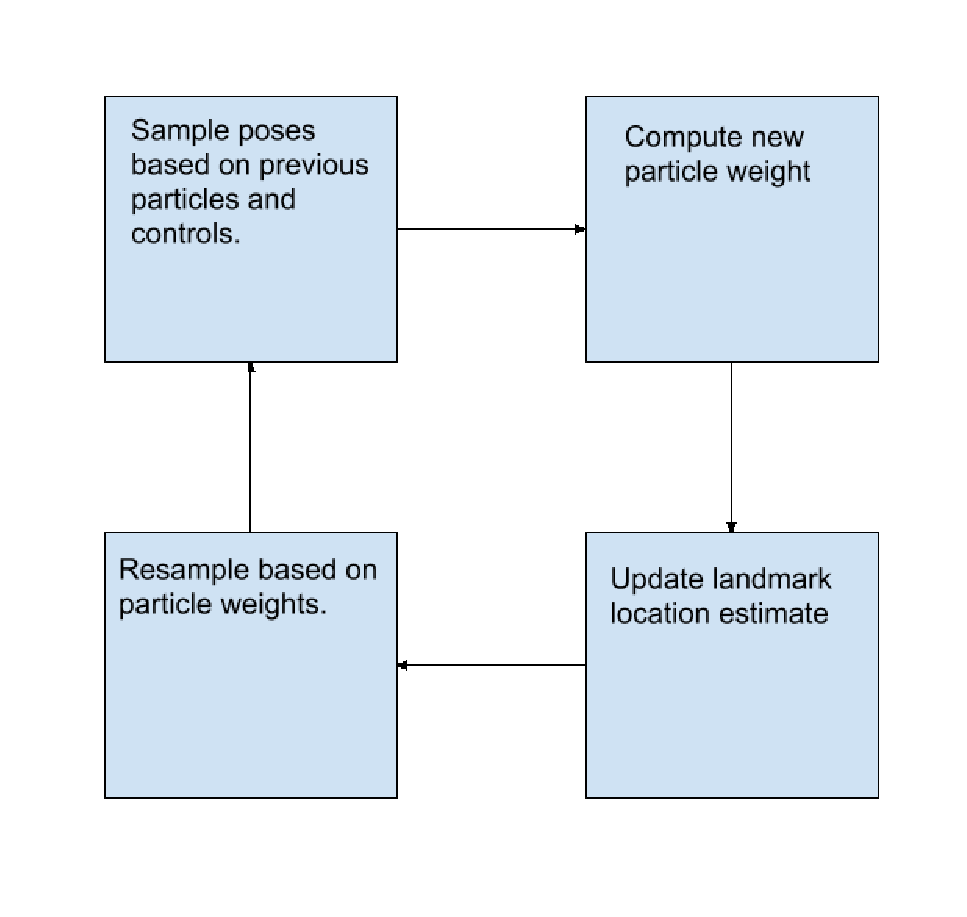
\includegraphics[width=7cm]{images/FastSLAMflow}
\end{figure}

\paragraph{Loop Closure and Localization}
%detecting loop closure and EKF localization
Loop closure will occurred as the vehicle finishes the first lap on the track. The purpose of loop closure is to minimize the accumulated error. Because of the high accuracy of DGPS, the vehicle will be able to accurate estimate when it has come back to its starting point. Additionally, because the starting point will be marked with different colored and sized cones, we will receive a signal once this particular cone is detected by the camera or lidar. In order to avoid a false positive case, (assuming loop closure immediately after the vehicle takes off) we will implement a state machine, the state machine will contain 3 states, the initial state would be set up when the car is ready to launch, after the car starts moving, it will transfer to second state that indicates the car is moving. Once the car is located within a certain range of the start point, it will transfer to its terminated state and a loop closure would be occurred only at terminated state. After the loop closure is detected, the map of the highest weighted particle will be selected and will no longer update. We will only take input from odometry and observations from camera and lidar, then we will implement an EKF on our observations in order to update the location of the vehicle.
\begin{figure}[H]
    \centering
    \caption{State Machine}
    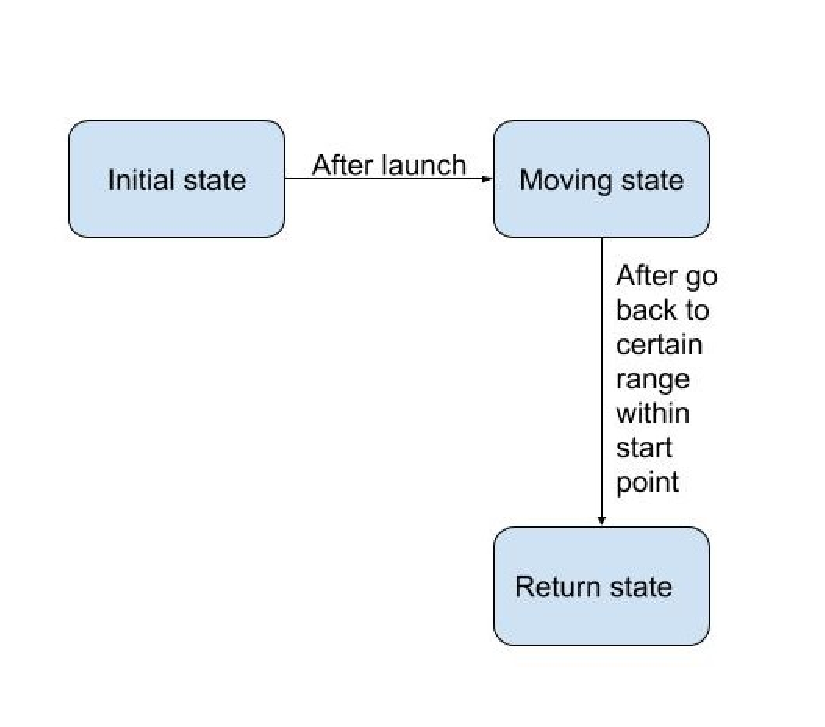
\includegraphics[width=7cm]{images/State_Machine}
    \label{fig:State_Machine}
\end{figure}

\paragraph{FastSlam Improvement}
%This section should outline the changes we will make from the Germans fastslam_1 to fastslam_2
For the first implementation of our SLAM algorithm we will be using FastSLAM1.0. The purpose being to produce a simple system quickly in order to begin testing and create a working model. We will then upgrade to FastSLAM2.0 after the initial implementation of FastSLAM1.0 has been evaluated. This upgrade is difficult since the implementation is much more complex, however, the end result will allow us to create more accurate and robust map and localization with fewer particles. Speed and accuracy are the primary criteria we are basing the SLAM design decisions upon and FastSLAM2.0 can produce higher accuracy with less data while decreasing the time spent updating sensor inputs.  

Loop closure's accuracy also improves; since FastSLAM2.0 data has a smaller error distribution, the ability to recognize a loop closure (i.e. data points it has already processed and mapped) is much higher. This difference becomes more evident as the loop increases in size. 

\begin{figure}[H]
\centering
\label{fig:FastSLAM1.0vFastSLAM2.0}
\caption{FastSLAM1.0 v FastSLAM2.0}
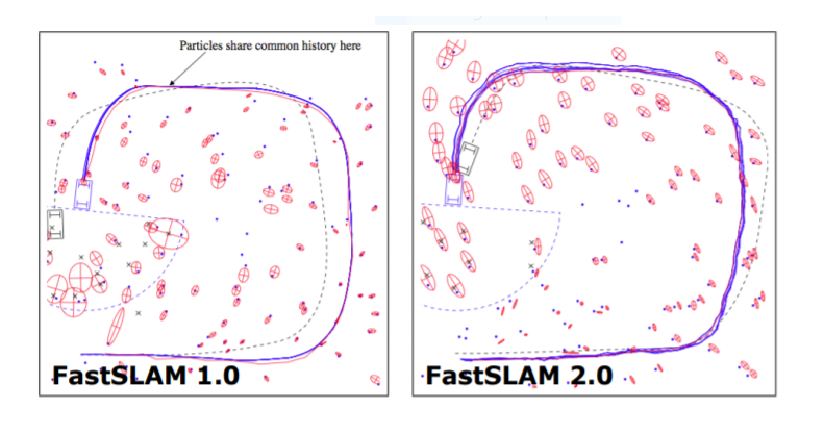
\includegraphics[width=10cm]{images/FastSLAM_1vFastSLAM_2}
\end{figure}


\subsubsection{Design Rationale} % Rationale behind our Design Element above (Why we chose the above implementation)
\paragraph{Open Loop SLAM}
FastSLAM was chosen for open loop SLAM because of its ability to handle non-linear distributions. The extended Kalman filter was considered because of how commonly it's used, but was not chosen because its accuracy relies on linear distributions and Gaussian noise. FastSLAM, while not as commonly used as the Kalman filter, still provides plenty of sources to draw from to help implement our own SLAM system.

\paragraph{Loop Closure and Localization}
An extended Kalman filter was chosen for the closed loop localization. An EKF was chosen because of its computational simplicity. In closed loop, the track is already recorded, so mapping cones is not the purpose of this system. Instead, EKF works to localize the car within the map. A particle filter may have been more robust for non-liner models, but keeping track of a high number of particles becomes computationally expensive.

\subsubsection{Design Tools} % What languages/packages/frameworks are used to accomplish our Design Element above
The SLAM system will be built in ROS along with the rest of the project components. ROS was chosen because of its ability to send data between nodes easily. The code for SLAM will be written in C++. ROS supports C++ and Python, but C++ was chosen because it has less overhead than Python. The Eigen C++ library will be used in the SLAM system to simplify matrix operations.

\nocite{*}
\bibliography{empty}

\end{document}

